% TODO: ARREGLAR JERARQUIA DE LAS MANOS

\section{Cambio de mano}

Antes de nada, voy a explicar la composición de las manos y de la espada en la escena:

\begin{itemize}
\item \textbf{Manos: }Están formadas por una esfera, que simula las manos, y un cilindro, que simula el antebrazo. Cabe destacar que para facilitar su animación, he realizado una jerarquía en la que las manos son el padre de los antebrazos.

En un modelo jerárquico tendría más sentido que el antebrazo fuese el padre, pero al estar animada nada más que la mano, he preferido que sea al revés para más facilidad a la hora de realizar ajustes en la animación.

\item \textbf{Espada: }La espada la he realizado utilizando como empuñadura un cilindro, un cubo achatado como guarda y para la hoja una pirámide de base rectangular y estirado en el eje Z para que sea más alto y puntiagudo.

\bigskip

Todas estas piezas las he agrupado para que sea más fácil trabajar con ellas. No obstante, al agrupar las piezas, el pivote se ha movido a la hoja, haciendo que cuando la agarre la mano no sea realista. Por tanto, es necesario mover el pivote de la espada de nuevo a la empuñadura.

\begin{figure}[H]
    \centering
    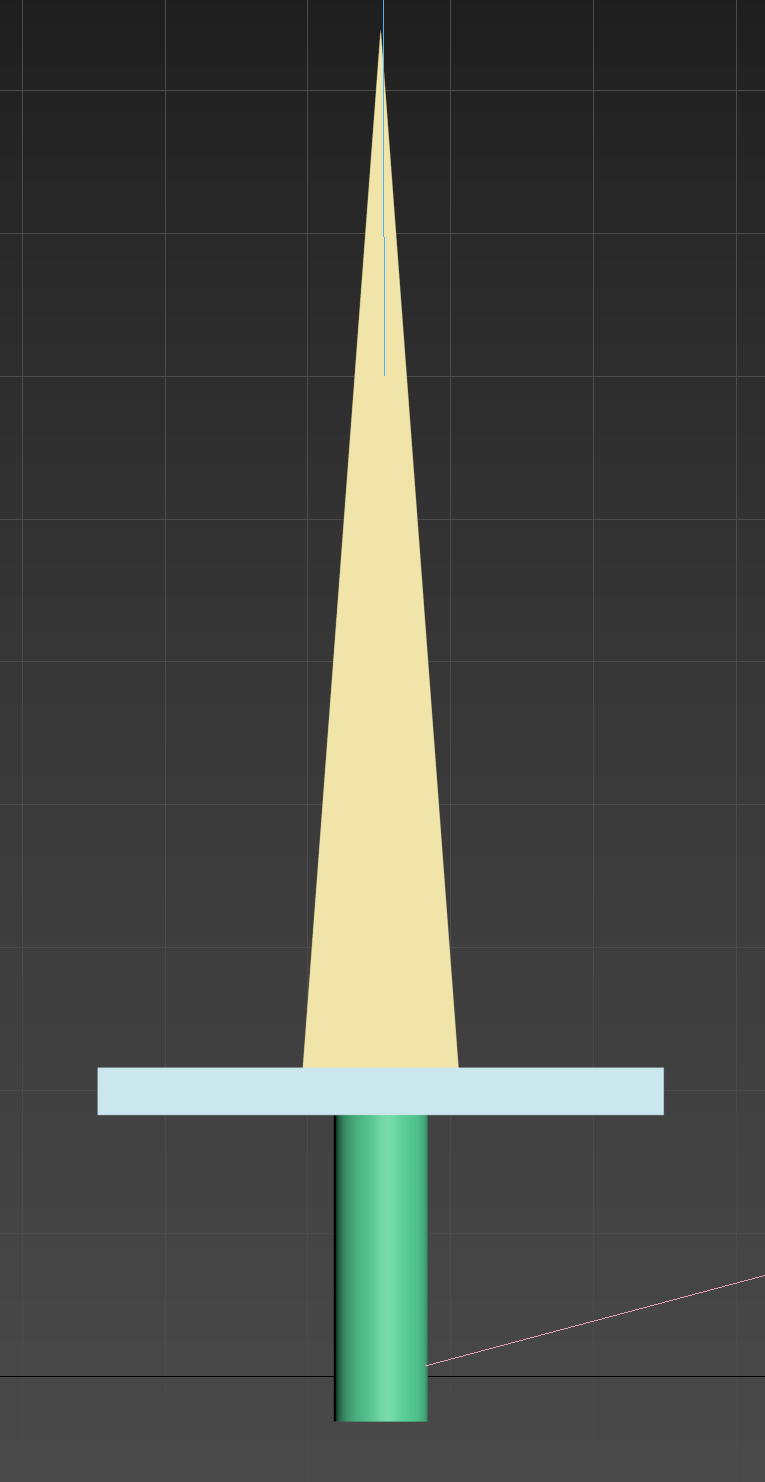
\includegraphics[width=0.2\textwidth]{imagenes/espada.png}
    \caption{Forma final de la espada.}
\end{figure}
\end{itemize}

\bigskip

Voy a dividir la configuración de las manos y de la espada en distintas subsecciones.

\subsection{Configuración de las manos}

Para la animación del cambio de mano, he utilizado los siguientes \textit{keyframes} para la mano más a la izquierda de la escena:

\begin{itemize}
    \item \textbf{Instante 0: }La mano se encuentra en su posición inicial, alejada de la otra mano.
    \item \textbf{Instante 20: }La mano se ha acercado a la otra para darle la espada.
\end{itemize}

Las curvas de la animación son:

% curvas
\begin{figure}[H]
   \centering
   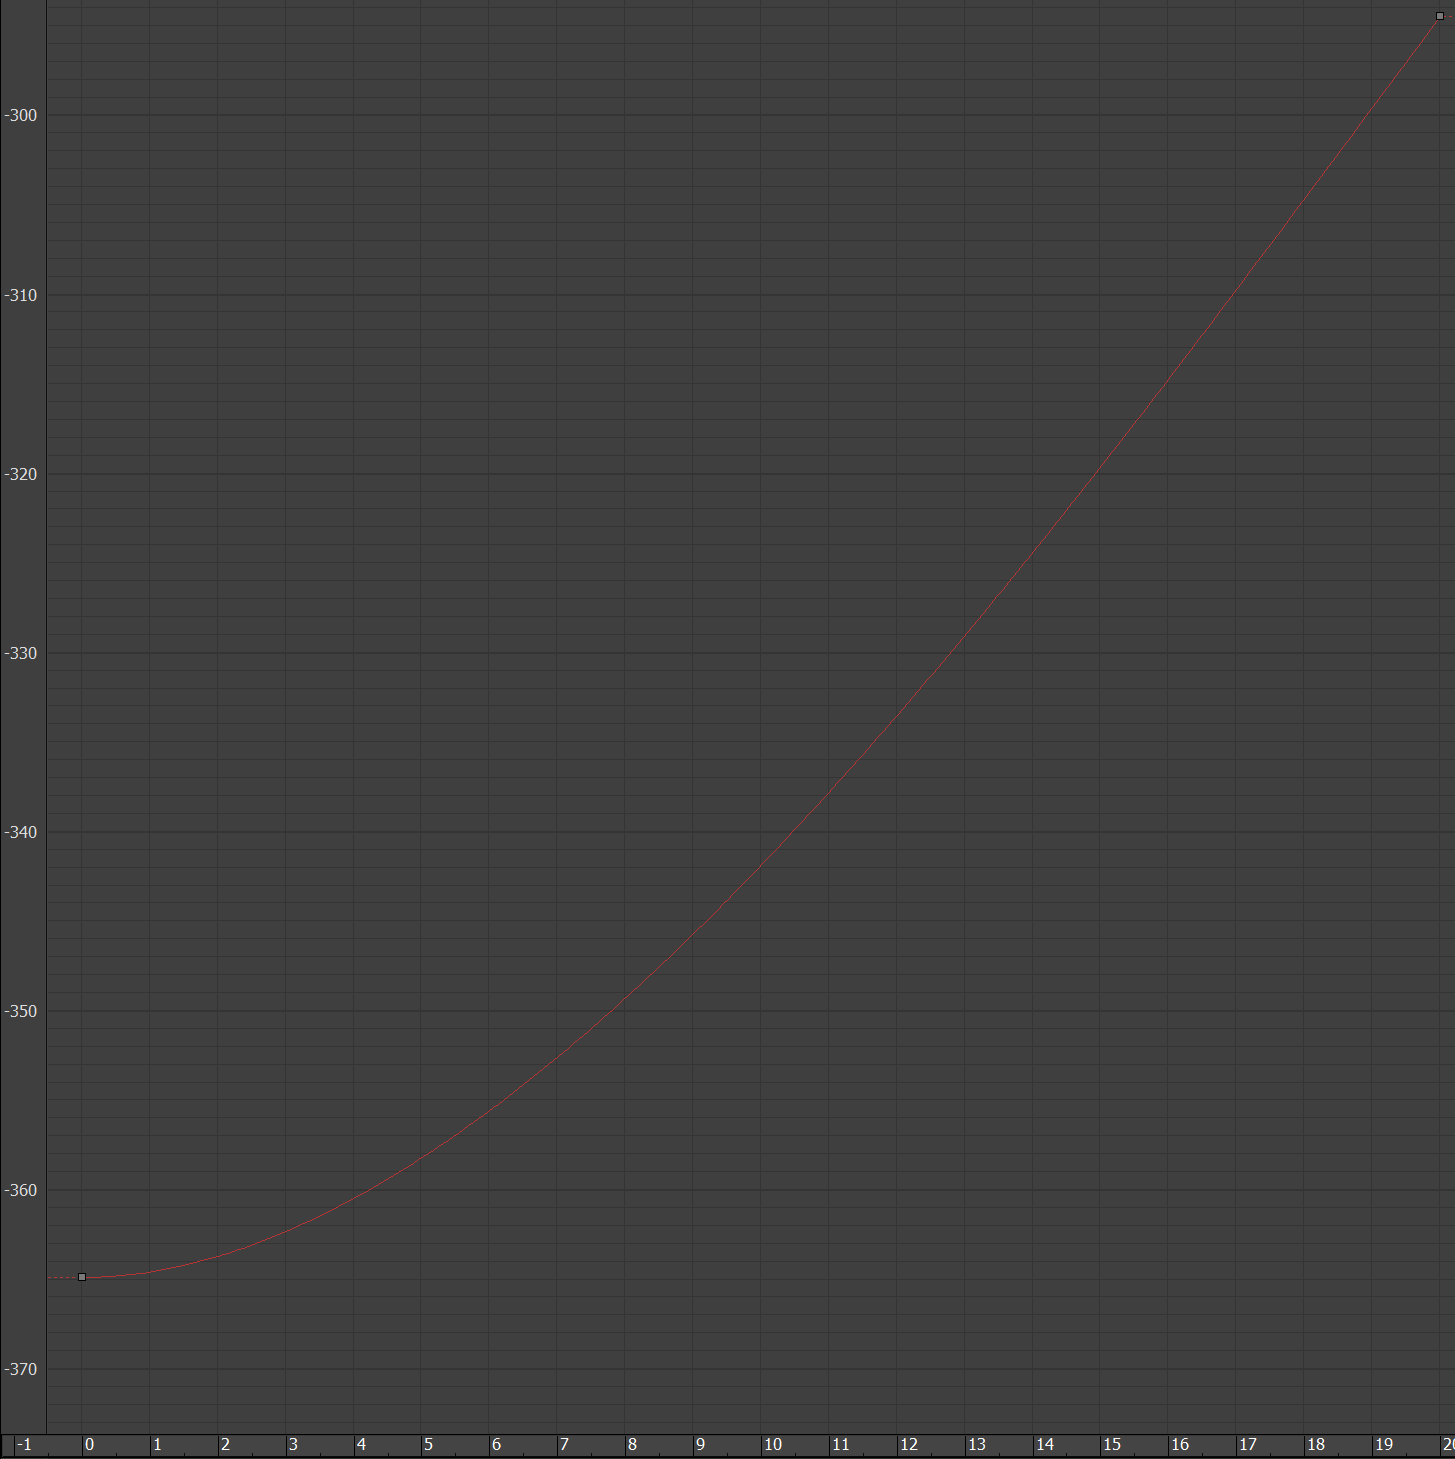
\includegraphics[width=0.6\textwidth]{imagenes/manos/izquierda/posX.png}
   \caption{Curva que representa la posición en el eje X de la mano izquierda.}
\end{figure}


% Como se puede ver, en todas las curvas he usado la forma por defecto \textit{Slow-in/Slow-out}, ya que genera unos resultados más orgánicos y acordes a estas extremidades.

Como se puede observar, he usado una curva de aceleración al principio, para simular la aceleración necesaria que requiere la mano y para intentar representar que la mano le ha lanzado la espada a la otra. Gracias a esta curva, se le puede transferir la velocidad a la espada de manera más o menos realista.

\bigskip


Mientras que la animación para la mano más a la derecha de la escena es: 

\begin{itemize}
    \item \textbf{Instante 30: }La mano se encuentra en su posición inicial y ha recibido la espada de la otra mano.
    \item \textbf{Instante 65: }Ahora la mano se ha dirigido a la plataforma de abajo de la grúa para dejar la espada.
    \item \textbf{Instante 70: }La mano se encuentra en la misma posición, encima de la plataforma. Esto lo he hecho así para simular la espera asociada a abrir la mano para dejar la espada.
    \item \textbf{Instante 90: }Finalmente la mano vuelve a la posición inicial.
\end{itemize}

Las curvas de animación para esta mano son:

\begin{figure}[H]
   \centering
   % curvas
   \begin{subfigure}[t]{0.32\textwidth}
       \centering
       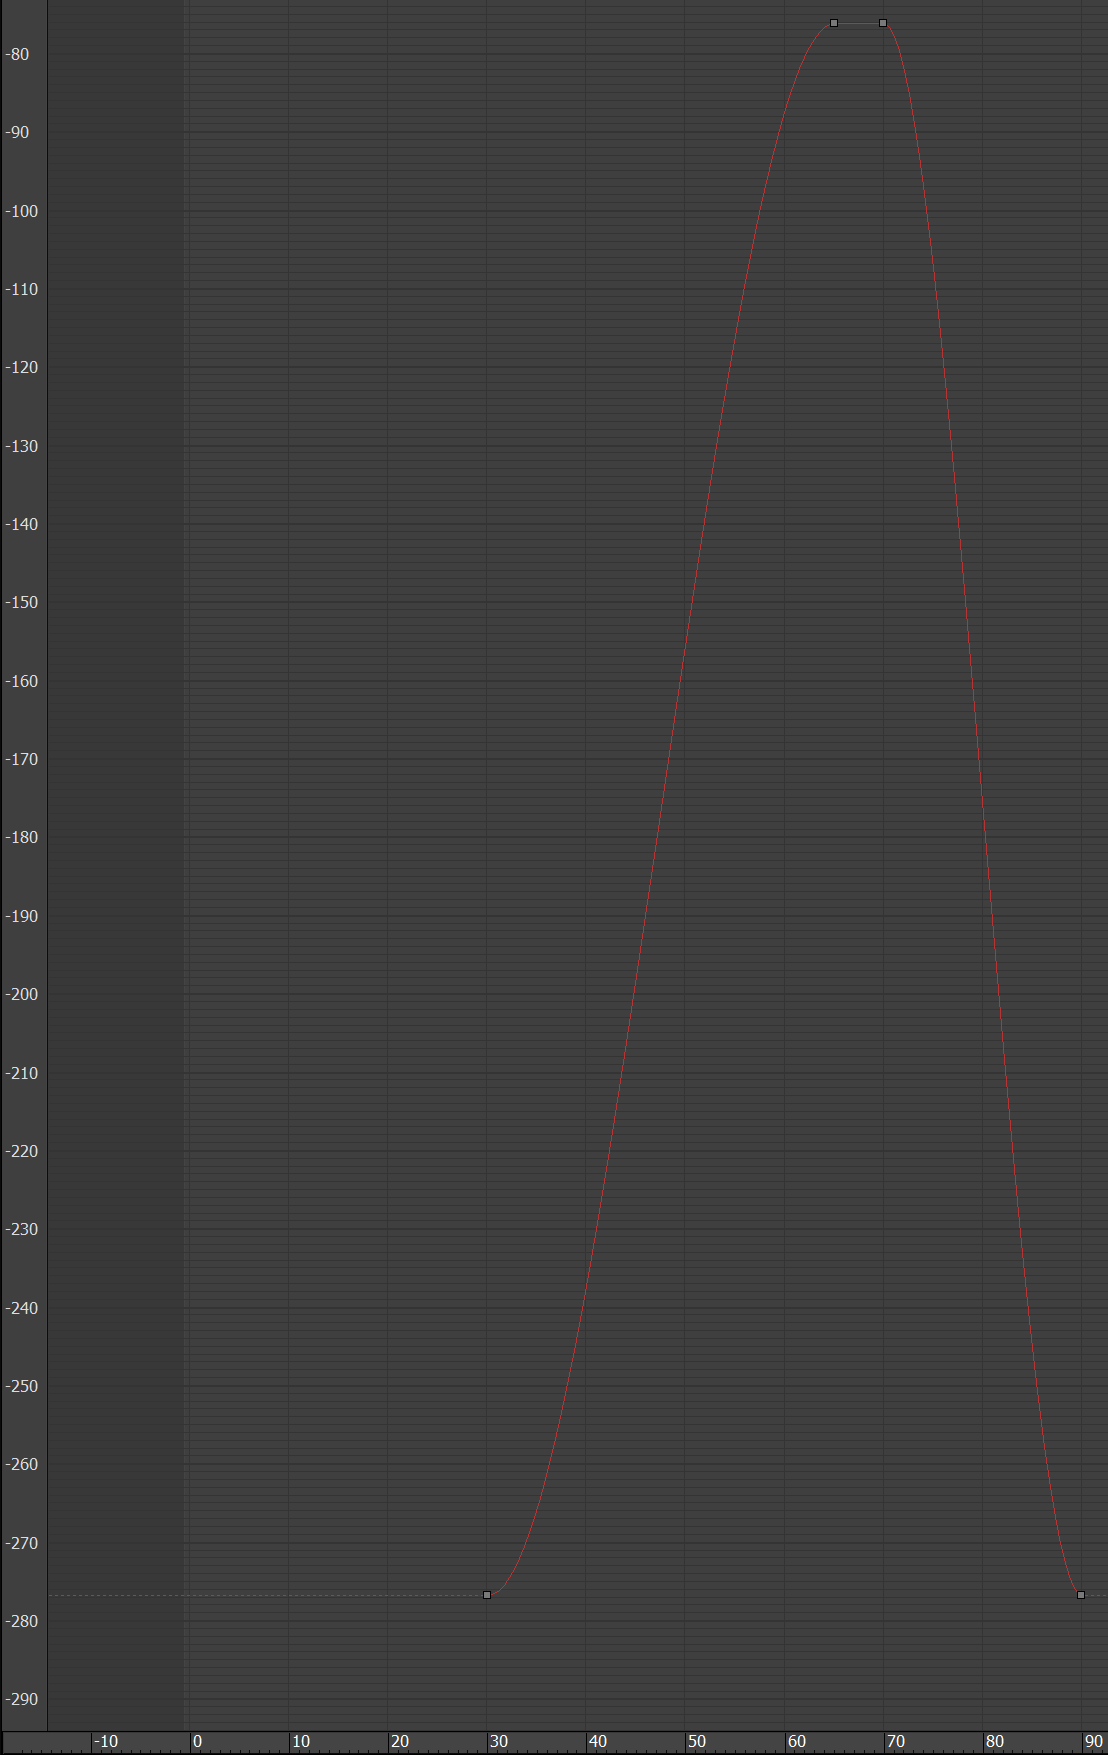
\includegraphics[width=\textwidth]{imagenes/manos/derecha/posX.png}
       \caption{Curva que representa la posición en el eje X de la mano derecha.}
    \end{subfigure}
   \hfill
    \begin{subfigure}[t]{0.32\textwidth}
       \centering
       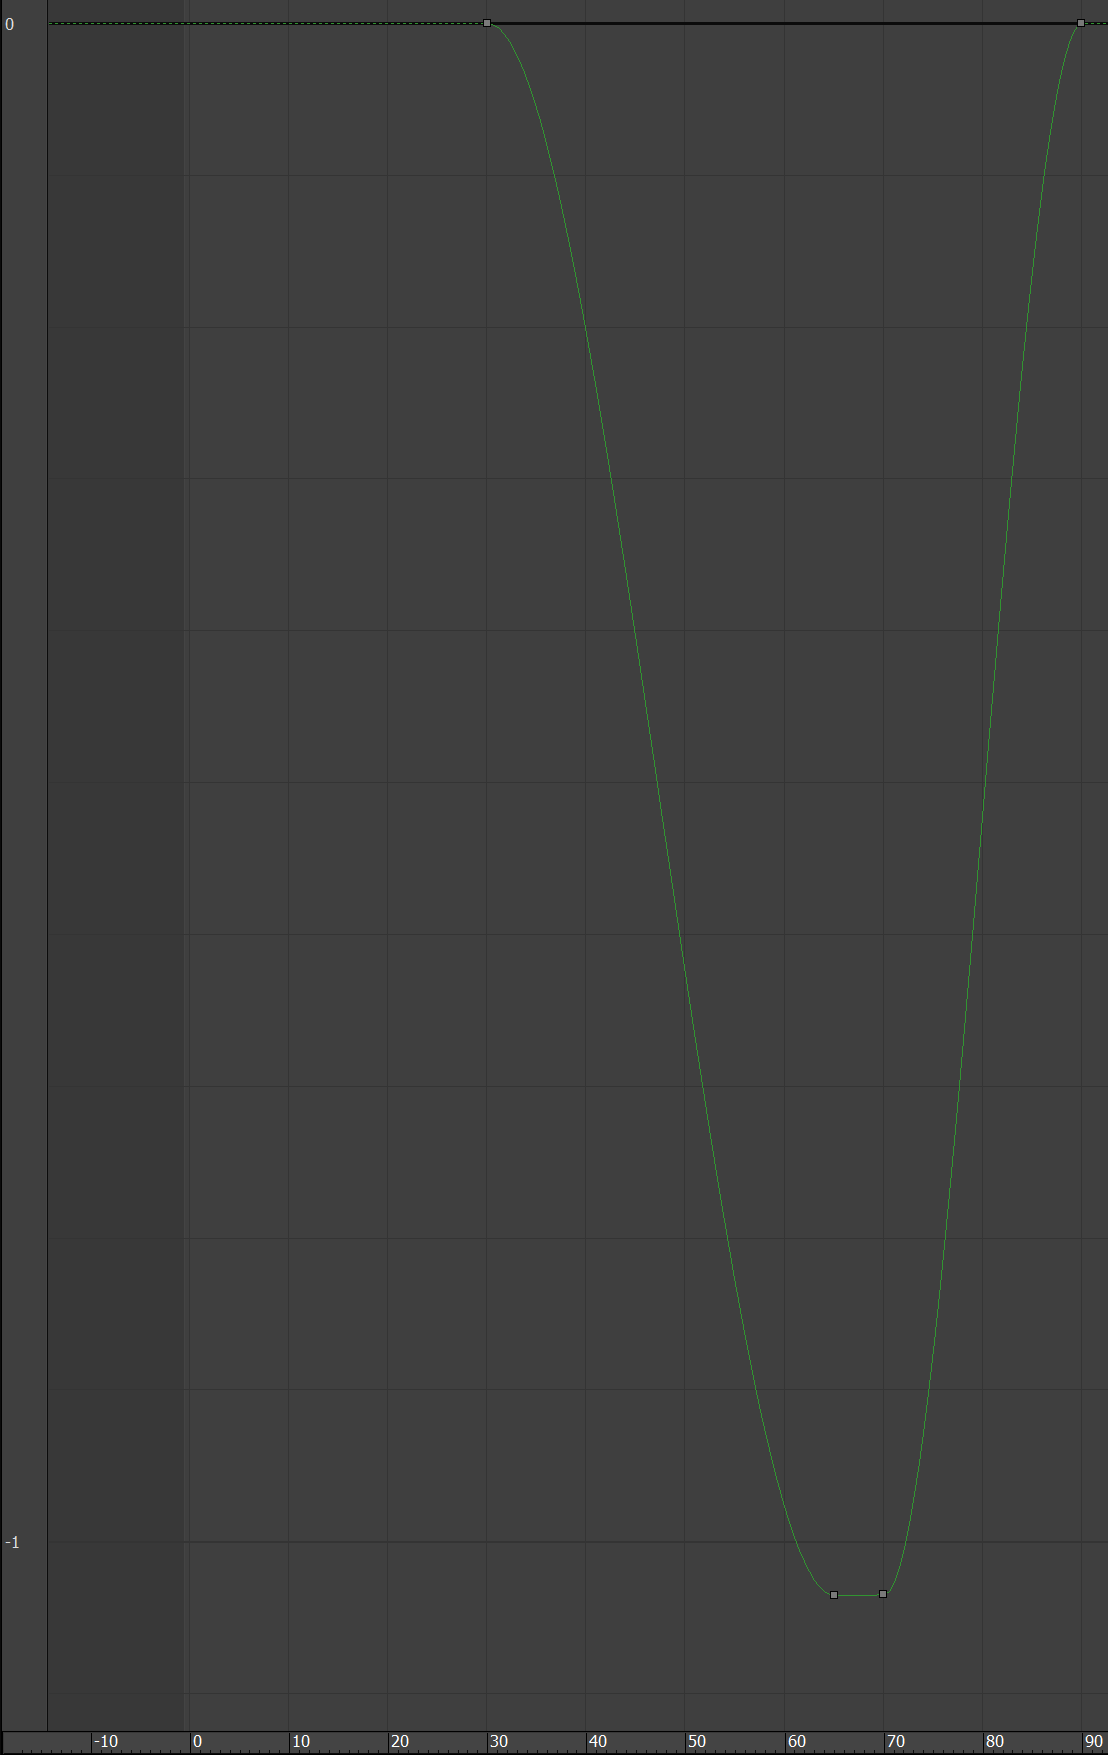
\includegraphics[width=\textwidth]{imagenes/manos/derecha/posY.png}
       \caption{Curva que representa la posición en el eje Y de la mano derecha.}
    \end{subfigure}
   \hfill
    \begin{subfigure}[t]{0.32\textwidth}
       \centering
       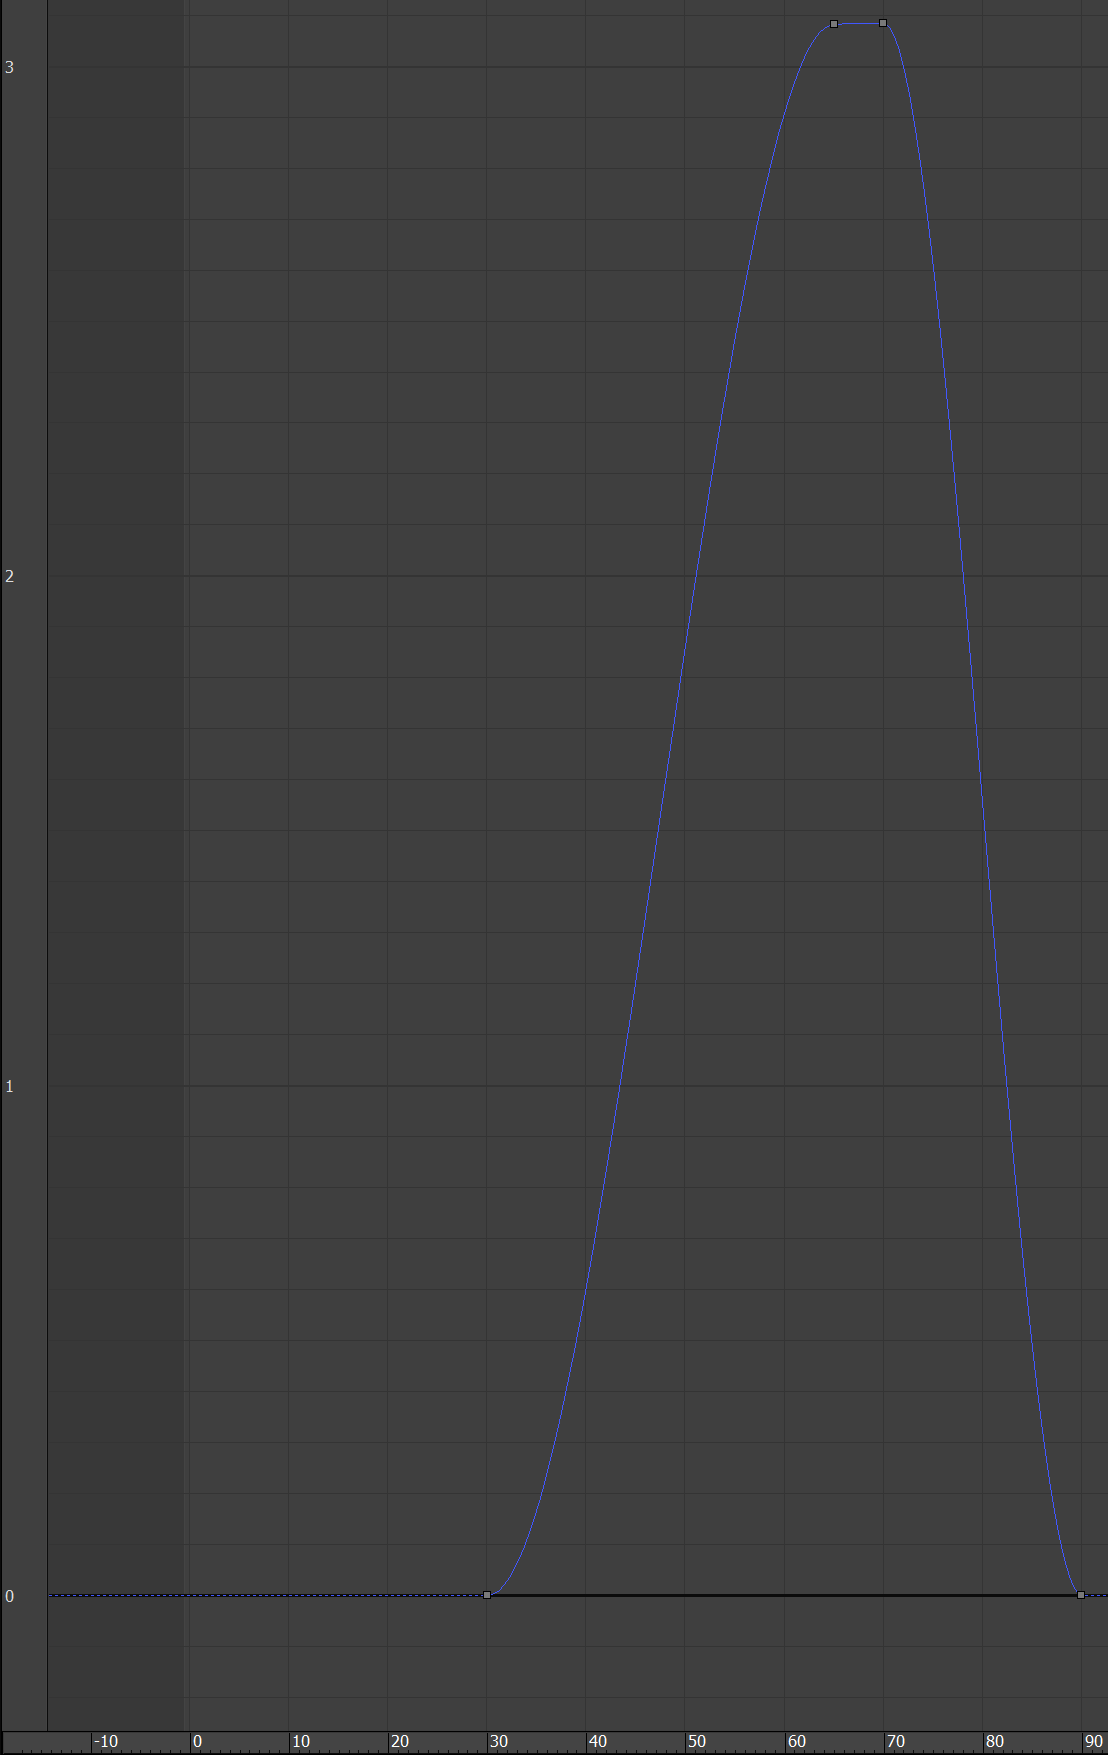
\includegraphics[width=\textwidth]{imagenes/manos/derecha/posZ.png}
       \caption{Curva que representa la posición en el eje Z de la mano derecha.}
    \end{subfigure}
    \caption{Curvas de animación de la mano derecha.}
\end{figure}


% De nuevo, se puede ver que en todas las curvas se ha utilizado la misma forma que para la otra mano, para dar un resultado más realista. 
En esta mano he utilizado la curva por defecto \textit{Slow-in/Slow-out} para todas las curvas, ya que da un resultado convincente, sobre todo cuando debe parar para dejar la espada en la plataforma, que desacelera progresivamente, similar a como se haría en la realidad.

\bigskip

Además, se puede observar como hay una animación en el eje Z. Esto es debido a que la plataforma se encuentra ligeramente más alta que los brazos, haciendo que este tenga que subir un poco y luego bajar para llegar a su posición inicial. Se podría haber bajado la plataforma un poco, para estar a la misma altura ambas, pero me di cuenta demasiado avanzado en el proceso y he preferido hacer este arreglo.

\bigskip

En cuanto a restricciones, ambas manos no tienen restricción de ningún tipo, es la espada la que tiene restricciones.


\subsection{Espada}

% HABLAR SOLO DE LA RESTRICCION DE POSICION, LA OTRA VA EN EL COCHE

La espada tiene dos restricciones, pero en esta sección solo voy a hablar de la de posición, que es la que le corresponde. En la sección del coche hablaré sobre la restricción de rotación.

\bigskip

Para animar el seguimiento de la espada en las manos y las plataformas, se debe hacer con un \textit{Position Constraint} o un \textit{Link}. En mi caso he usado el primero, que por defecto solo afecta al canal de la posición.

\bigskip

Después, he elegido como \textit{targets} las manos y la plataforma, animando después el cambio de pesos. El peso inicialmente estará en la mano más a la izquierda de la escena, después estará en la otra mano y finalmente todo el peso se encontrará en un \textit{dummy} que hay en la plataforma.

% foto de los pesos
\begin{figure}[H]
    \centering
    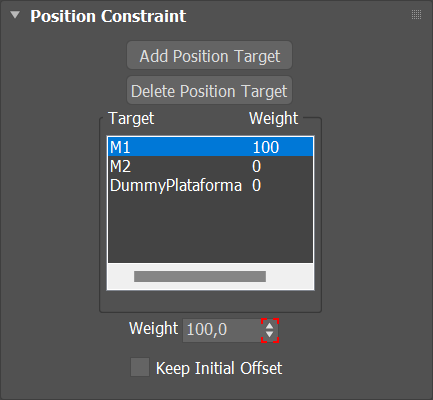
\includegraphics[width=0.4\textwidth]{imagenes/espada/pesosPC.png}
    \caption{Objetivos utilizados para esta restricción.}
 \end{figure}

Los \textit{keyframes} referentes a este \textit{constraint} son:

\begin{itemize}
    \item \textbf{Instante 20: }Todo el peso se encuentra en la mano izquierda inicialmente.
    \item \textbf{Instante 27: }Ahora todo el peso se encuentra en la otra mano.
    \item \textbf{Instante 65: }No hay ningún cambio, el peso sigue encontrándose en la mano derecha.
    \item \textbf{Instante 70: }El peso ahora se encuentra en el \textit{dummy} de la plataforma.
\end{itemize}

\bigskip

En cuanto a la curva de animación referente al \textit{Position Constraint} es la siguiente:

% curva de animacion
\begin{figure}[H]
   \centering
   % curvas
   \begin{subfigure}[t]{0.27\textwidth}
       \centering
       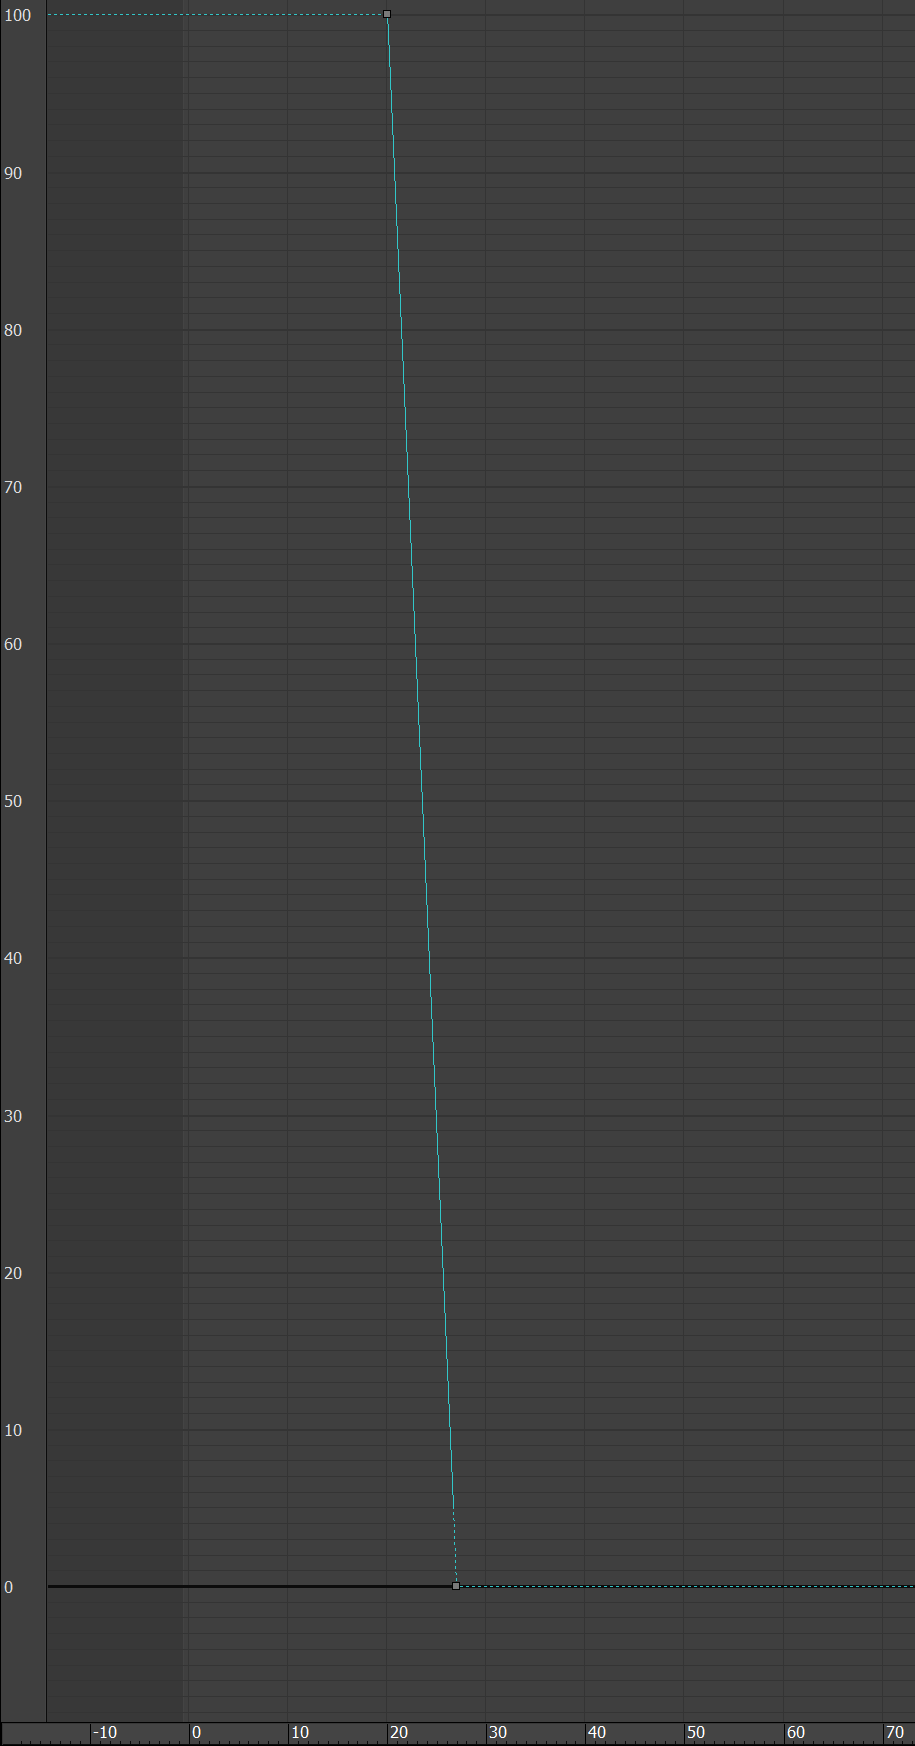
\includegraphics[width=\textwidth]{imagenes/espada/peso0.png}
       \caption{Curva que representa el peso de la mano izquierda con respecto al tiempo.}
    \end{subfigure}
   \hfill
    \begin{subfigure}[t]{0.27\textwidth}
       \centering
       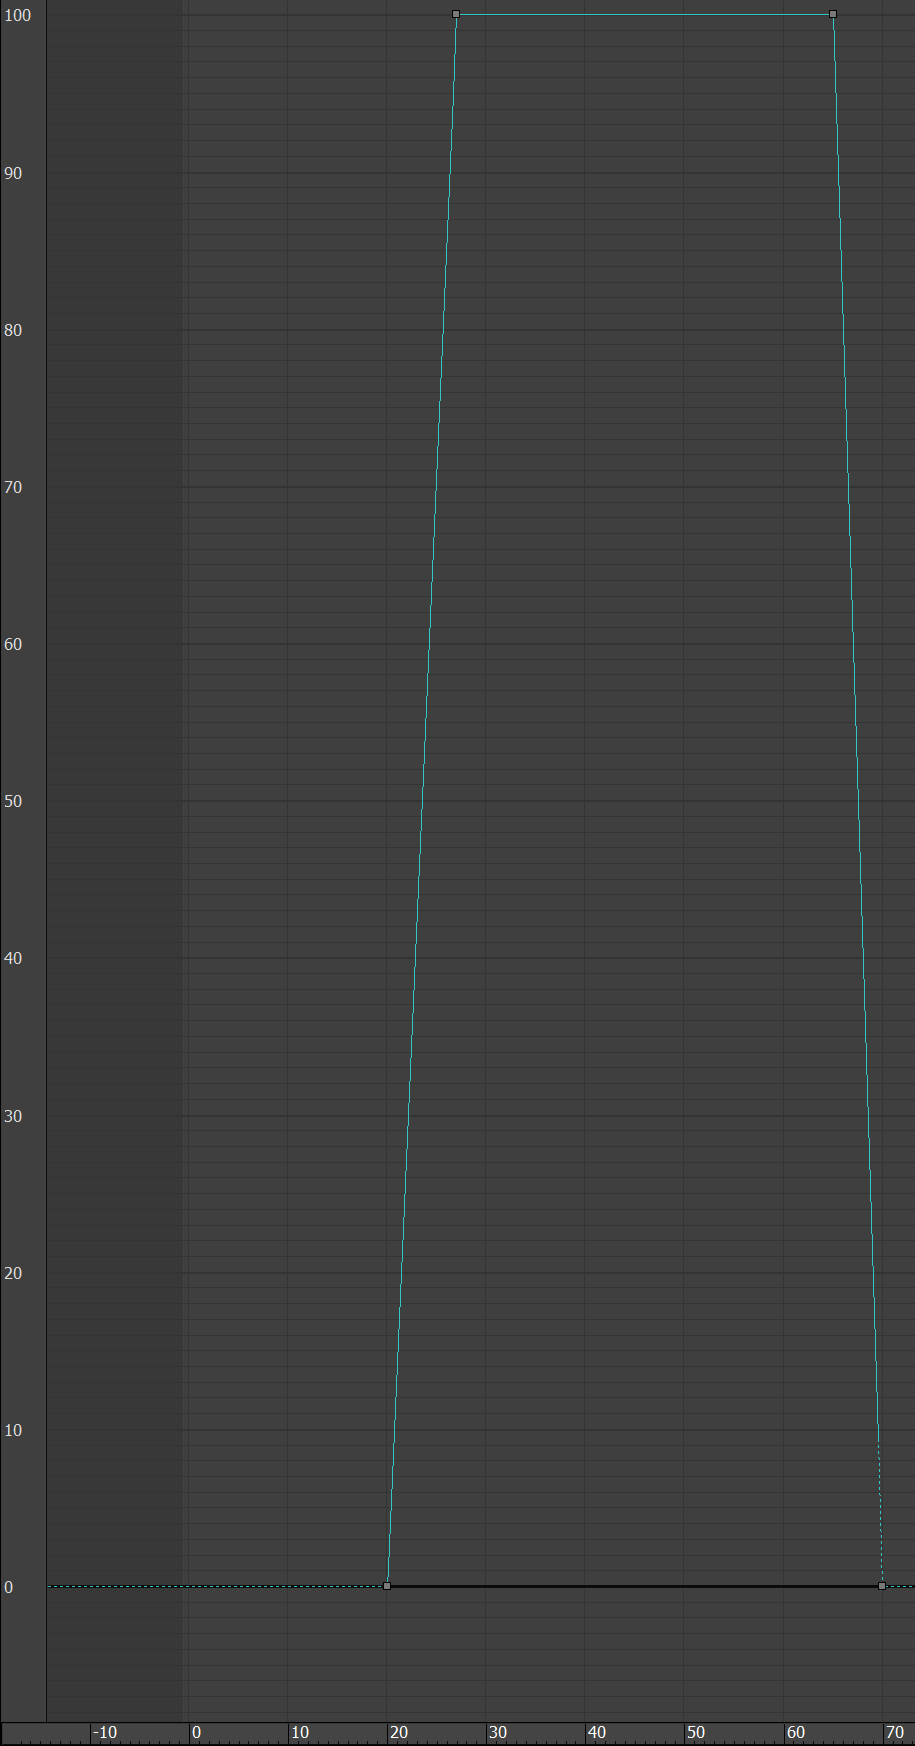
\includegraphics[width=\textwidth]{imagenes/espada/peso1.png}
       \caption{Curva que representa el peso de la mano derecha con respecto al tiempo.}
    \end{subfigure}
   \hfill
    \begin{subfigure}[t]{0.27\textwidth}
       \centering
       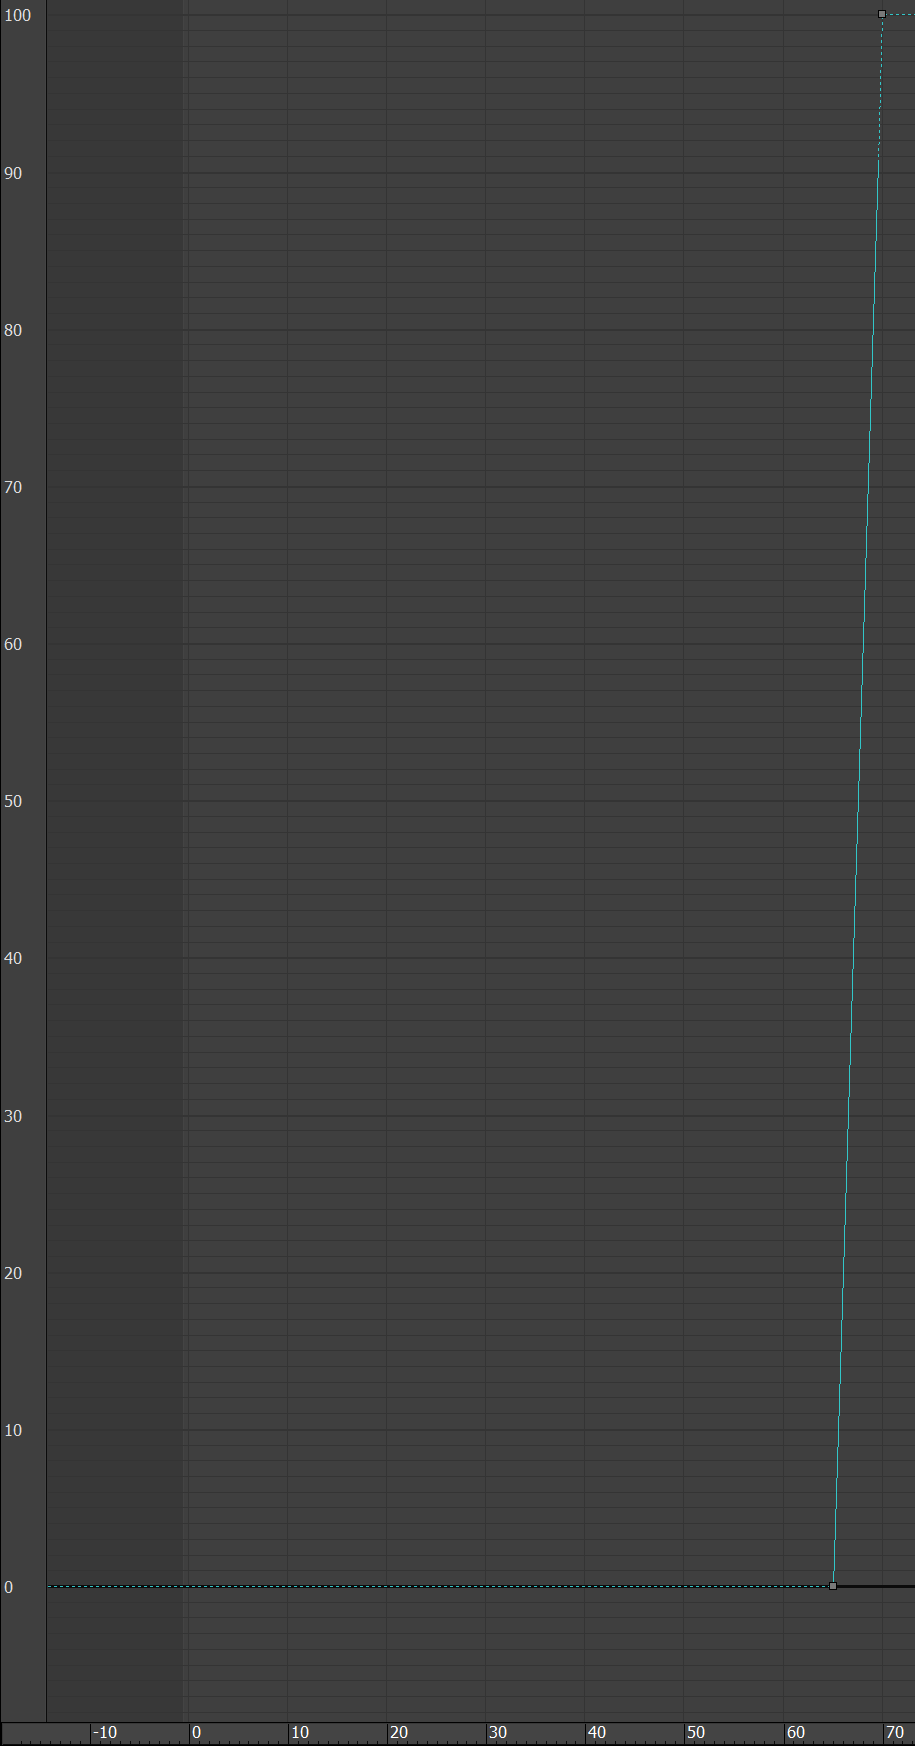
\includegraphics[width=\textwidth]{imagenes/espada/peso2.png}
       \caption{Curva que representa el peso de la plataforma con respecto al tiempo.}
    \end{subfigure}
    \caption{Curvas de los pesos del \textit{Position Constraint}.}
\end{figure}

Como se puede observar, las curvas de animación son lineales. Lo he hecho así para simular el lanzamiento de la espada de la mano izquierda, que le transfiere su velocidad. El paso de la mano derecha a la plataforma lo he hecho de forma lineal también, ya que la mano se posa sobre el siguiente punto en el que debe estar la espada, haciendo que esta no se mueva y no se aprecie diferencia entre distintos tipos de curva.

\bigskip

La configuración del \textit{Position Constraint} es:

\begin{figure}[H]
   \centering
   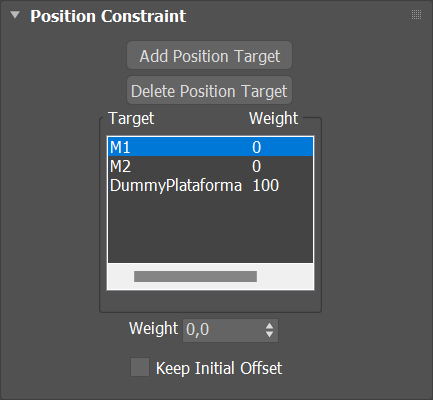
\includegraphics[width=0.4\textwidth]{imagenes/espada/PCconfig.png}
   \caption{Configuración final del \textit{Position Constraint}.}
\end{figure}

\subsection{Resultado final en el cambio de manos}

El resultado final de todo esto es el siguiente:

% fotos de los fotogramas mas importantes.
\begin{figure}[H]
   \centering
\begin{subfigure}[t]{0.48\textwidth}
    \centering
    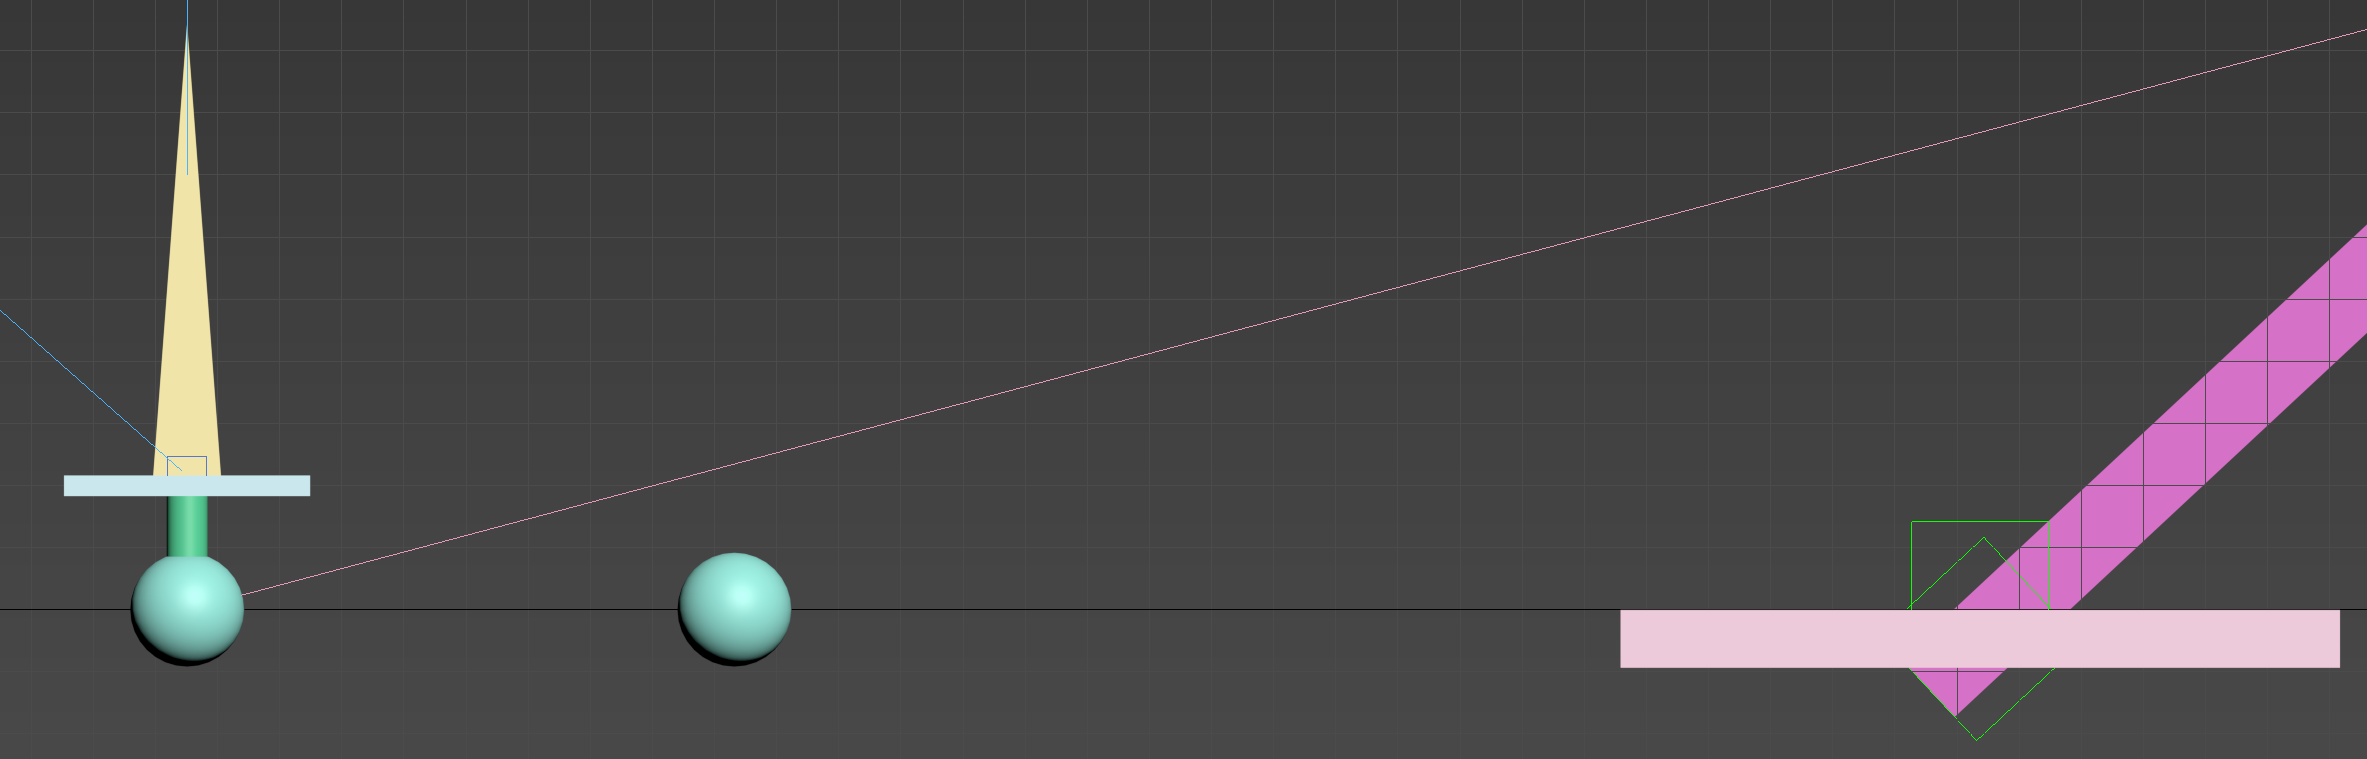
\includegraphics[width=\textwidth]{imagenes/espada/keyframes/0.png}
    \caption{Manos en el instante 0.}
 \end{subfigure}
\hfill
 \begin{subfigure}[t]{0.48\textwidth}
    \centering
    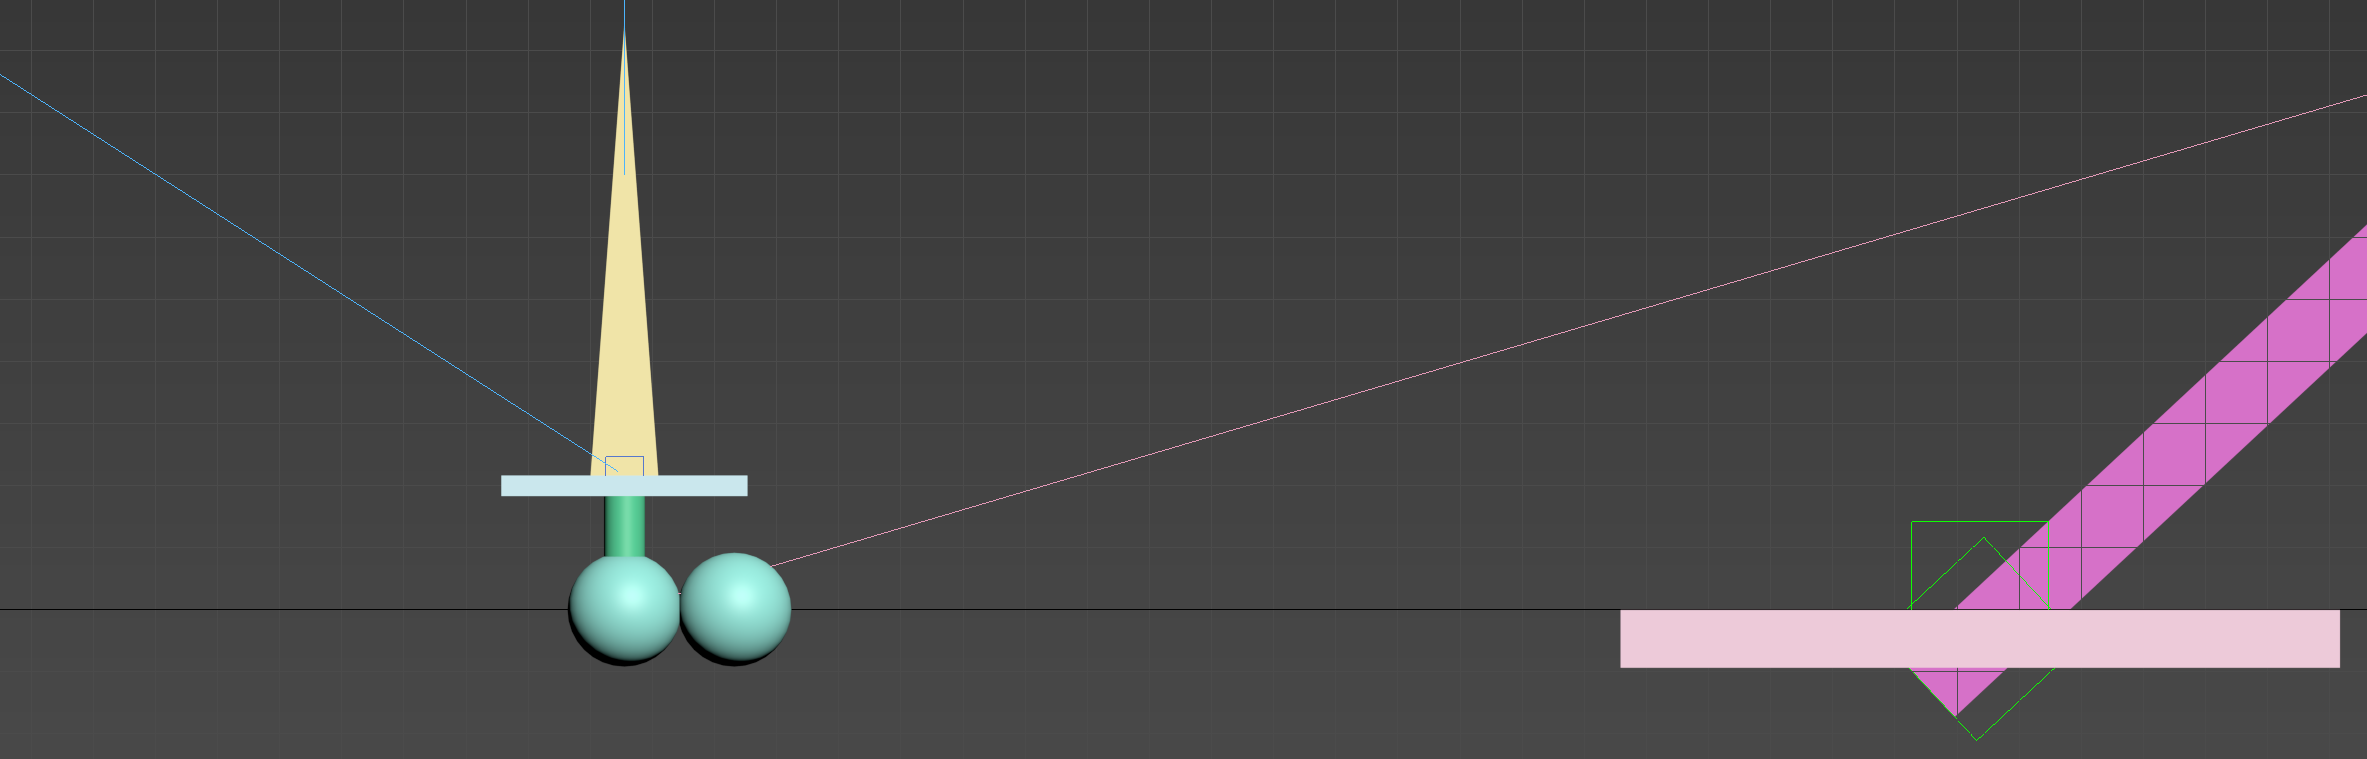
\includegraphics[width=\textwidth]{imagenes/espada/keyframes/20.png}
    \caption{Manos en el instante 20.}
 \end{subfigure}
\hfill
 \begin{subfigure}[t]{0.48\textwidth}
    \centering
    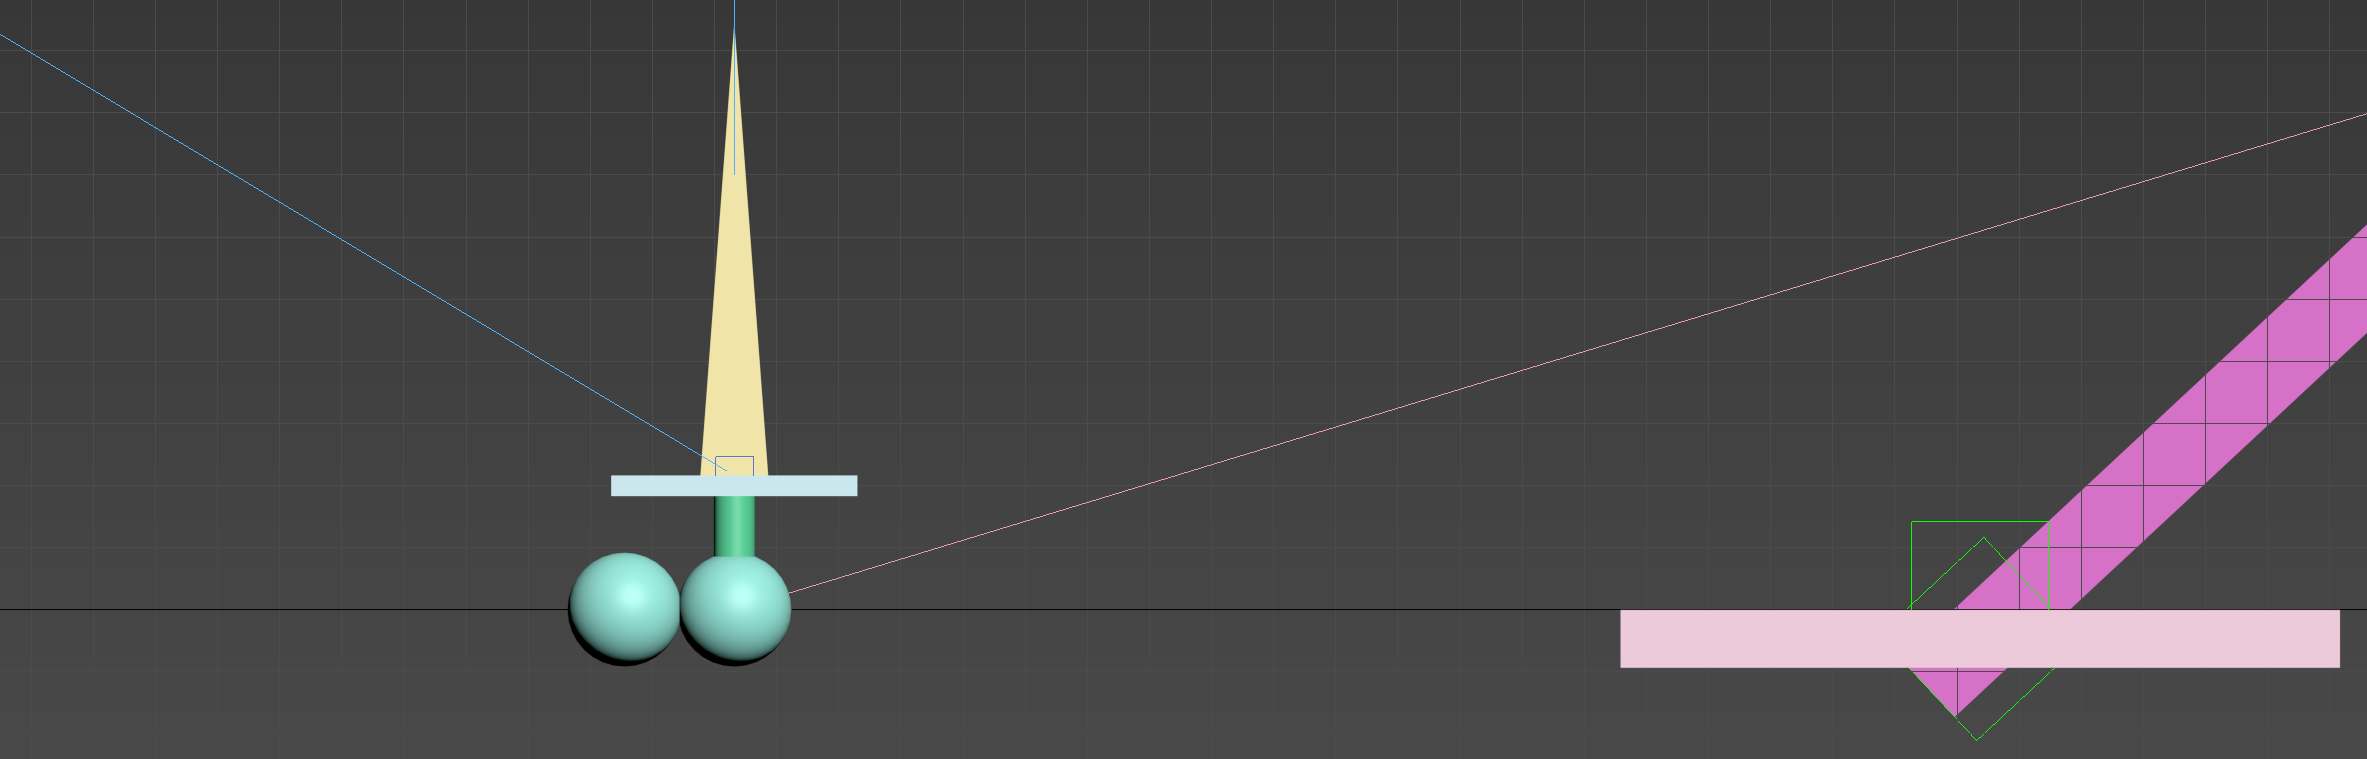
\includegraphics[width=\textwidth]{imagenes/espada/keyframes/27y30.png}
    \caption{Manos en los instantes 27 y 30.}
 \end{subfigure}
\hfill
 \begin{subfigure}[t]{0.48\textwidth}
    \centering
    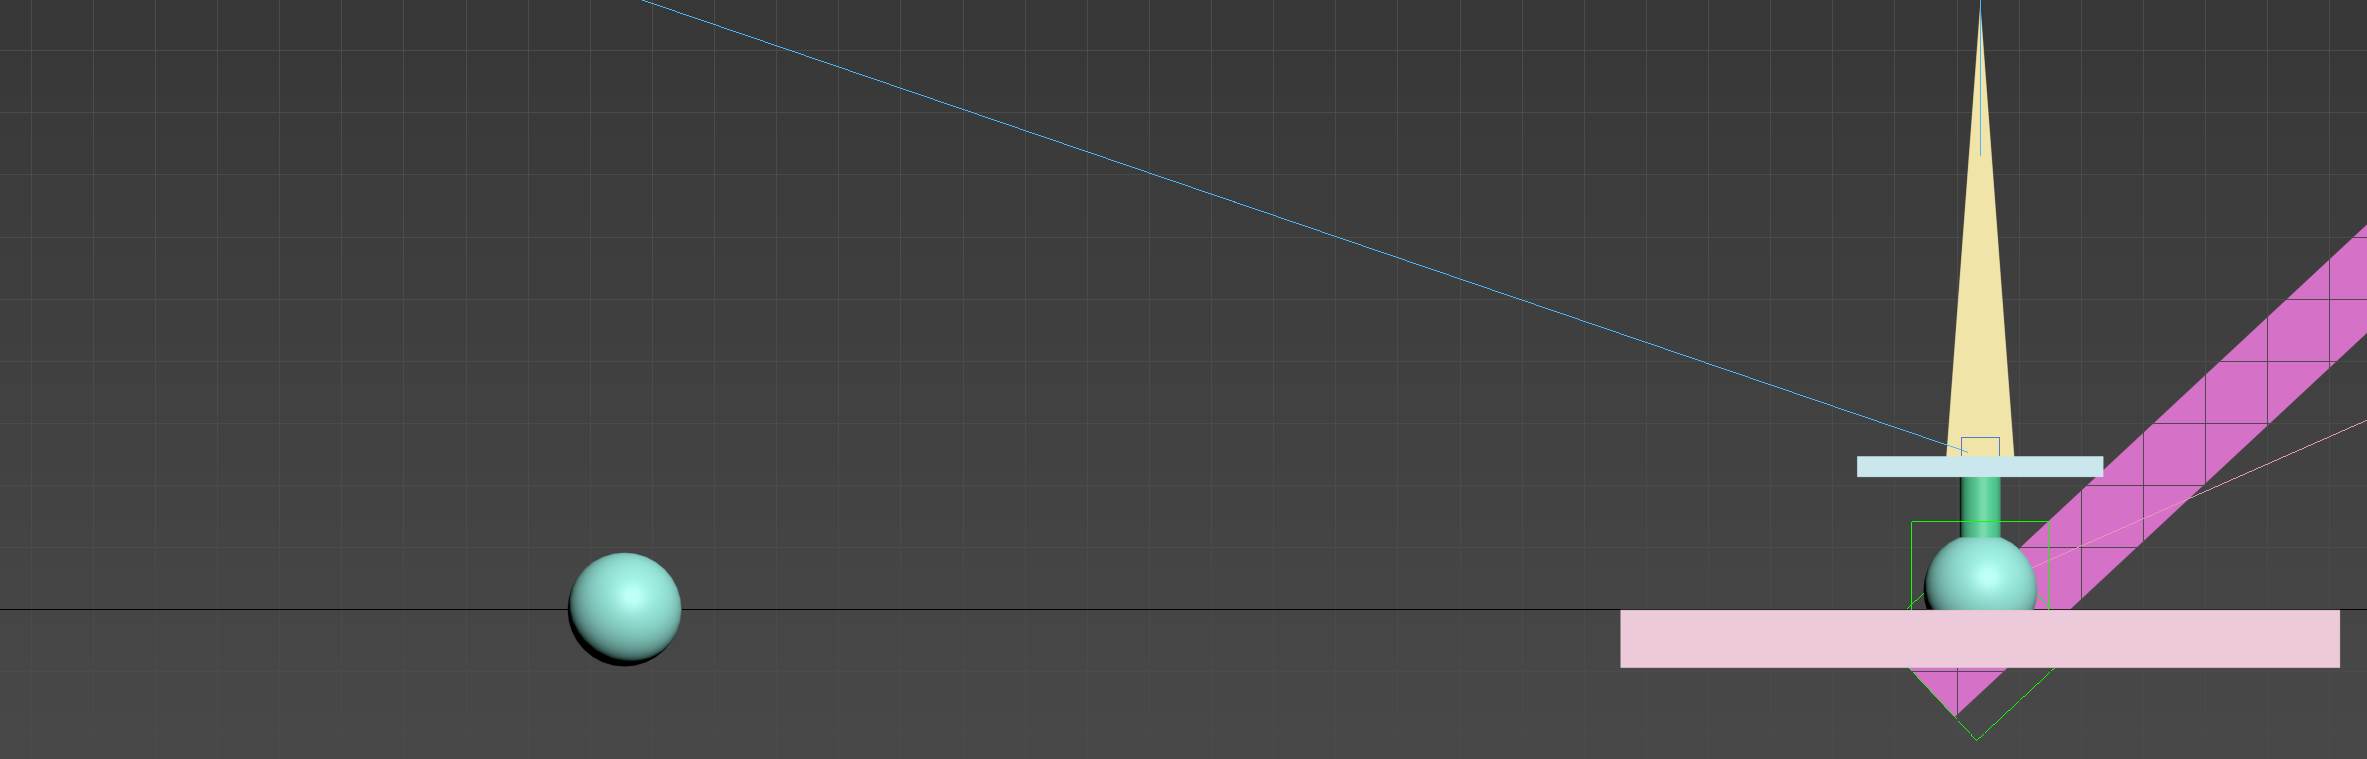
\includegraphics[width=\textwidth]{imagenes/espada/keyframes/65y70.png}
    \caption{Manos en los instantes 65 y 70.}
 \end{subfigure}
\hfill
 \begin{subfigure}[t]{0.48\textwidth}
    \centering
    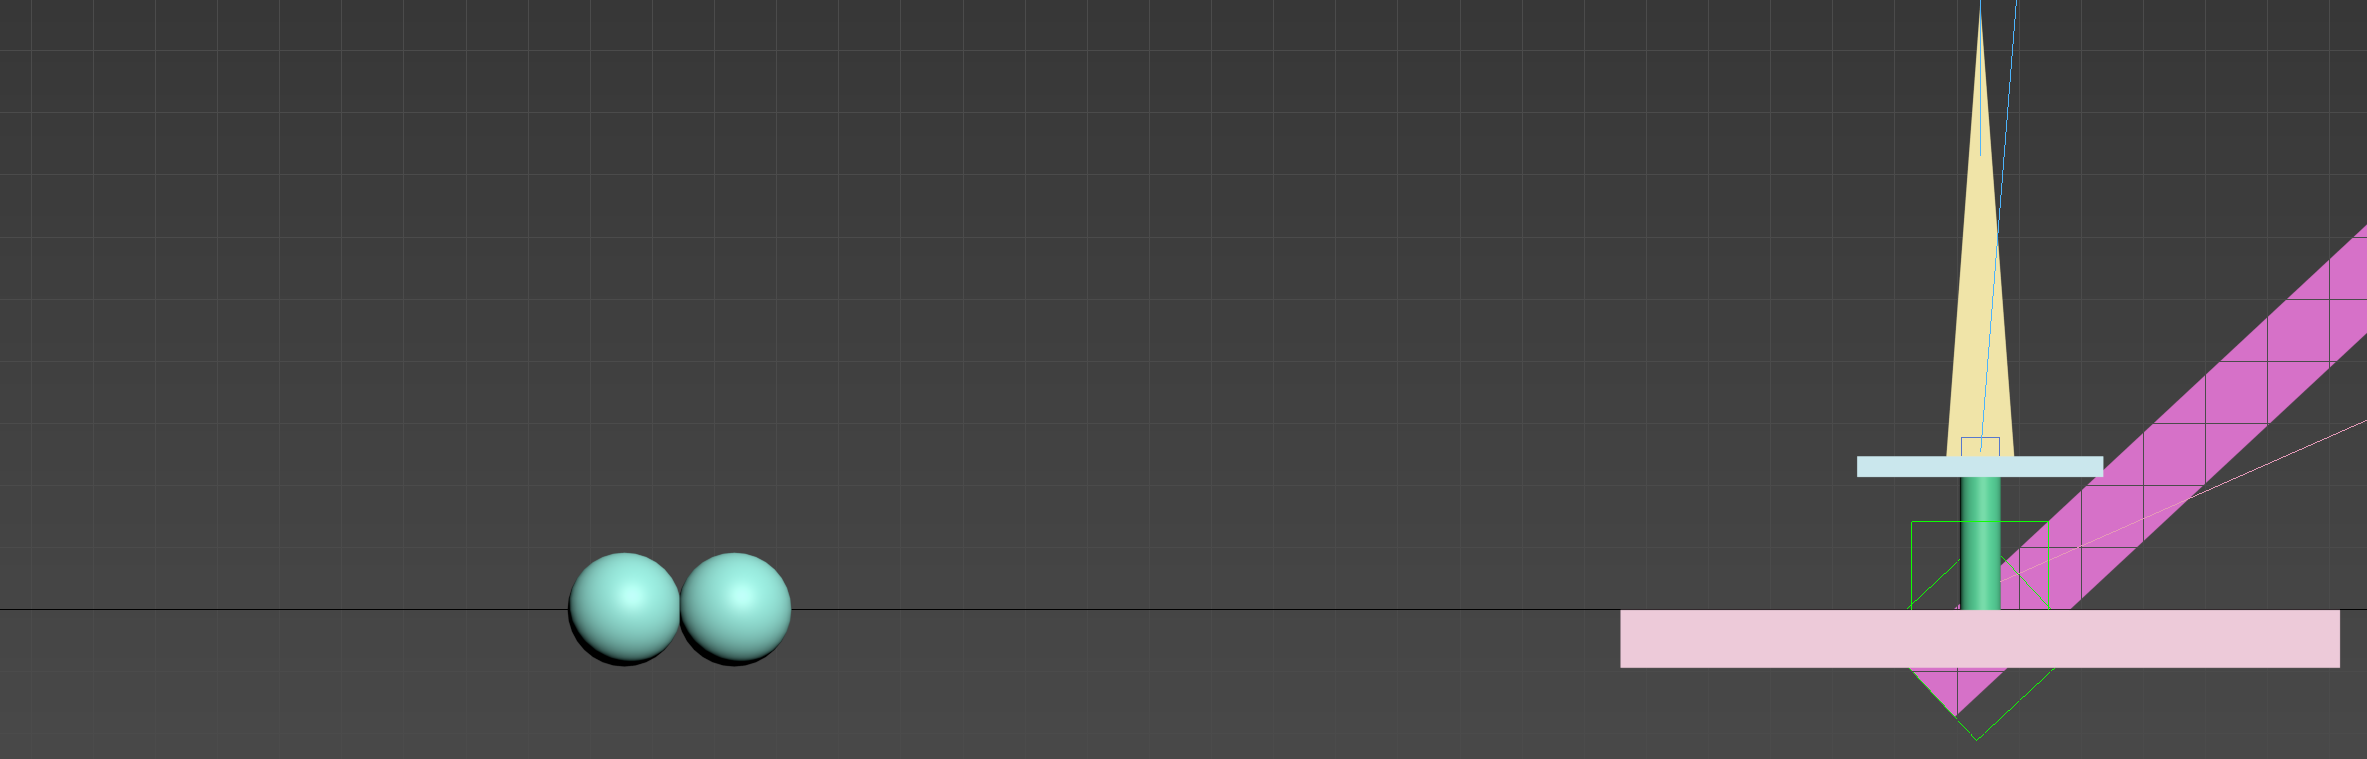
\includegraphics[width=\textwidth]{imagenes/espada/keyframes/90.png}
    \caption{Manos en el instante 90.}
 \end{subfigure}
 \caption{\textit{Keyframes} más importantes de la animación de las manos.}
\end{figure}